\documentclass{article}
\usepackage[top=1in, bottom=1.5in, left=1.2in, right=1.2in]{geometry}
\title{\textbf{Maximizando o Desempenho de Portfólio Através do Índice Sharpe}}
\author{Grupo 8 - Gustavo Barroso Souza Cruz, Ian Cordibello Desponds}
\date{\today}
\usepackage{graphicx}
\usepackage{afterpage}
\usepackage{amsmath}

\begin{document}
    \maketitle
    \section*{Introdução ao Portfólio}
    
    O portfólio é estruturado de maneira fundamentada e coerente, justamente devido à sua adesão
     a princípios robustos e bem estabelecidos de gestão de ativos. Alicerçado na diversificação 
     eficiente, desempenho histórico consistente, um índice Sharpe substancial, a meticulosa 
     seleção de ativos e uma sólida compreensão do contexto econômico, 
    esse portfólio se destaca como uma estratégia de investimento inteligente e fundamentada.

    \subsection*{Diversificação}
    
    Primeiramente, a diversificação desempenha um papel crucial na construção desse portfólio
    . A inclusão de ativos de diferentes setores, como telecomunicações, mineração, varejo
     farmacêutico, medicina diagnóstica e automação industrial, é uma medida prudente para mitigar 
     riscos. Isso significa que o portfólio não está excessivamente concentrado em um único setor da economia, o que 
    reduz significativamente a exposição a flutuações abruptas de preços em um segmento específico.

    \subsection*{Desempenho Histórico}

    Além disso, o desempenho histórico notável do portfólio ao longo dos últimos cinco anos é indicativo de que as escolhas de 
    ativos foram acertadas. Embora seja essencial lembrar que o desempenho passado não é uma garantia de resultados futuros, a 
    consistência ao longo do tempo sugere que a estratégia de investimento aplicada até o momento tem sido bem-sucedida.

    \subsection*{Índice Sharpe}

    O índice Sharpe elevado, atingindo a notável marca de 68,58, é uma prova concreta de que o portfólio está gerando retornos 
    superiores em relação ao risco assumido. Essa métrica é fundamental para avaliar a eficácia da alocação de ativos e demonstra 
    que o portfólio está oferecendo uma recompensa substancial pelo risco incorporado.

    \subsection*{Seleção de Ativos}

    A seleção criteriosa de ativos também é um componente essencial desse portfólio. As empresas escolhidas, como a Telefônica, 
    Vale, Raia Drogasil, Fleury e Weg, são líderes em seus respectivos setores e possuem históricos de desempenho sólidos. Esse 
    rigor na seleção aumenta a confiança na capacidade dessas empresas de continuar a prosperar no ambiente de mercado.

    \section*{Conclusão}

    \subsection{Gráfico}
    \begin{figure}[h]
        \centering
        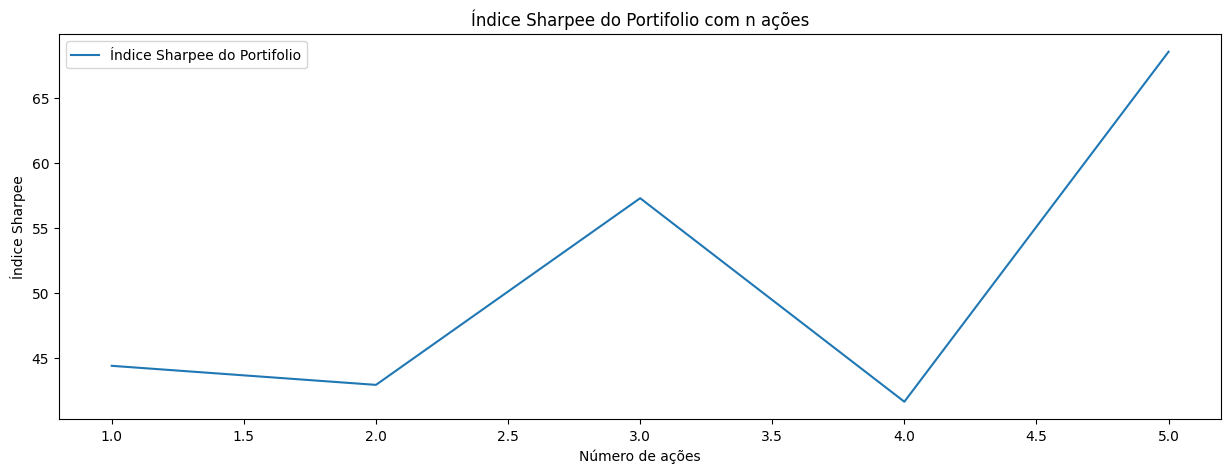
\includegraphics[width=0.9\textwidth]{shapee.png}
    \end{figure}

    Em síntese, o portfólio em questão é uma escolha coesa e bem embasada, cuja estrutura é sustentada pela aplicação de 
    princípios sólidos, como diversificação eficiente, desempenho histórico consistente, índice Sharpe elevado e uma seleção 
    criteriosa de ativos. Esses elementos, juntos, contribuem para a robustez e a eficácia da estratégia de investimento adotada, 
    refletindo uma abordagem informada e fundamentada no mundo dos investimentos.

    \subsection{Autoavaliação}

    Texto - Conceito A, porque nossa escolha de ações foi bem pensada, garantindo uma diversificação 
    do portfólio, além de serem ativos já estabelecidos no mercado, o que evita grande volatilidade nos 
    valores e proporciona um alto índice de sharpe e baixo risco.
    Gráfico - Conceito A, porque a figura representou a evolução do índice sharpe do portfólio à medida
    que ações são adicionadas, mostrando que o portfólio se torna mais eficiente e com menor risco.

\end{document}
